%sri

\section{Experiments}

\subsection{Index Tasks}

\paragraph{Growth of memory as execution proceeds}
\paragraph{Performance overhead as execution proceeds}


\begin{center}
 \begin{tabular}{||c | c | c | c||} 
 \hline
 NumIter& No Resilience & Resilience without -lf:resilience & Only lg:resilient \\ [0.25ex] 
 \hline\hline
128 & 23 & 16 & 21\\ 
 \hline
256 & 20 & 22 & 28\\ 
 \hline
512 & \\ [1ex] 
 \hline
\end{tabular}
\end{center}




\begin{center}
 \begin{tabular}{||c | c | c | c||} 
 \hline
 NumIter& No Resl No lg:res & No Res With lg:res & Res No lg:res \\ [0.25ex] 
 \hline\hline
100 &  7.2 & 6.6 & 23.6\\ 
 \hline
200 &  13.8 & 13.3 & 46.3\\ 
 \hline
400 &  26.1 & 26.5 & 94.4\\ 
 \hline
800 &  55 & 53 & 186.8\\ 
 \hline
1000 &  65 & 66 & 239.9\\ [1ex] 
 \hline
\end{tabular}
\end{center}

\begin{figure}
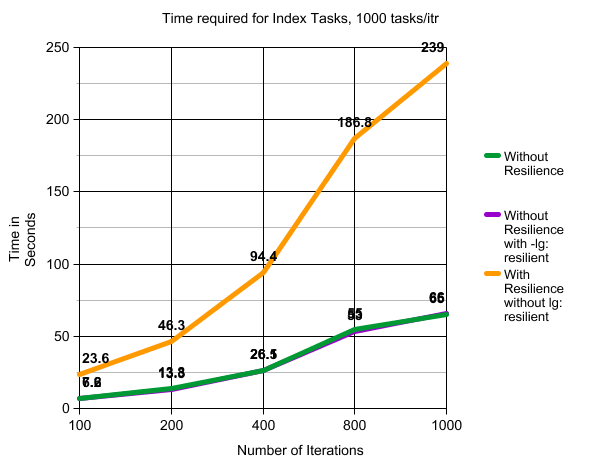
\includegraphics[width=\textwidth]{images/index_tasks_time.png}
\caption{Total time taken by 02\_index\_tasks. Time in Seconds, 1000 tasks/index launch }
\end{figure}

\begin{center}
 \begin{tabular}{||c | | c | c ||} 
 \hline
 NumIter& No Resilience & Resilience \\ [0.25ex] 
 \hline\hline
100 &  1.12 & 2.43\\ 
 \hline
200 &  1.56 & 4.39\\ 
 \hline
400 &  3.00 & 9.45\\ 
 \hline
800 &  5.58 & 19.09\\ 
 \hline
1000 &  7.34 & 23.2 \\ [1ex] 
 \hline
\end{tabular}
\end{center}

\begin{figure}
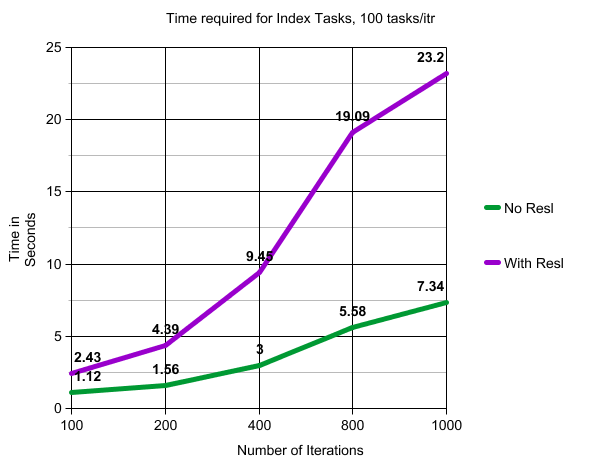
\includegraphics[width=\textwidth]{images/index_tasks_time2.png}
\caption{Total time taken by 02\_index\_tasks. Time in Seconds, 100 tasks/index launch }
\end{figure}




\begin{center}
 \begin{tabular}{||c | c | c | c||} 
 \hline
 NumIter& No Resl No lg:res & No Res With lg:res & Res No lg:res \\ [0.25ex] 
 \hline\hline
100 &  18 & 140 & 107 \\ 
 \hline
200 &  22 & 263 & 176 \\ 
 \hline
400 &  24 & 509 & 245 \\ 
 \hline
800 &  26 & 1002 & 428\\ 
 \hline
1000 & 26 & 1248 & 518\\ [1ex] 
 \hline
\end{tabular}
\end{center}

\begin{figure}
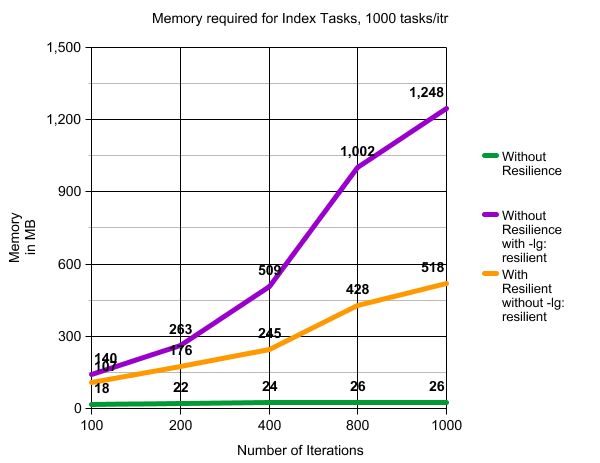
\includegraphics[width=\textwidth]{images/index_tasks_memory.png}
\caption{Total Memory footprint by 02\_index\_tasks. Memory in MB, 1000 tasks/index launch.}
\end{figure}





\subsection{Stencil}



\subsection{local recover vs global recovery}

\subsection{compute/comm vs no-failure/single failure/multi-failure}

\subsection{S3D, Pennant, Stencil, Circuit}

\subsection{Some Interesting Task Graphs for Recovery}

\subsection{bigger examples}
pennant, stencil, miniAero (better understood) /Circuit, 
- limit the failure to the before


